

Capturing behavior variations across inputs is important in the design
of an \FDO\ compiler. A number of speculative code transformations are
known to benefit from \FDO, including speculative partial redundancy
elimination~\cite{ChowChanPLDI97,GuptaICCL98}, trace-based
scheduling and others~\cite{BodikGuptaPLDI97,ChekuriMICRO96}.% Several
%open questions remain about the use of profiles collected from
%multiple runs of a program.  How should the multiple profiles be
%combined? Is it sufficient to simply average the multiple
%measurements? Is it necessary to compute the parameters for an assumed
%statistical distribution of the measurements? Or is there a simple
%technique to combine the measurements and provide useful statistics to
%\FDO?

This section argues that the behavior
variations in an application due to multiple inputs should be
evaluated by \FDO\ decisions.  It also argues that a full parametric
estimation of a statistical distribution is not only unnecessary, but
it may also mislead FDO decisions if the wrong distribution is assumed
or there is insufficient data to accurately estimate the
parameters.% Instead, it proposes the use of a non-parametric empirical
%distribution that makes no assumptions about the shape of the actual
%distribution. 


A major challenge in the use of traditional single-training-run \FDO\
is the selection of a profiling data input that is representative of
the execution of the program throughout its lifetime.  For large and
complex programs dealing with many use cases and used by a multitude
of users, assembling an appropriately representative workload may be a
difficult task.  Picking a solitary training run to represent such a
space is far more challenging, or potentially impossible, if use-cases
are mutually-exclusive.  While benchmark programs can be modified to
combine such use-cases into a single run %(\refSection{single:spec}),
this approach is obviously inapplicable to real programs.  Moreover,
user workloads are prone to change over time.  Ensuring stable
performance across all inputs in today's workload prevents performance
degradation due to changes in the relative importance of workload
components.

The {\em Combined Profiling} (\CP) statistical modeling technique
%presented in this chapter produces a {\it Combined Profile} (\CProf)
presented in ~\cite{BerubePhD} produces a {\it Combined Profile} (\CProf)
from a collection of traditional single-run profiles, thus
facilitating the collection and representation of profile information
over multiple runs. The use of many profiling runs, in turn, eases the
burden of training-workload selection and mitigates the potential for
performance degradation.  There is no need to select a single input
for training because data from any number of training runs can be
merged into a combined profile.  More importantly, \CP\ preserves
variations in execution behavior across inputs.  The distribution of
behaviors can be queried and analyzed by the compiler when making
code-transformation decisions.  Modestly profitable transformations
can be performed with confidence when they are beneficial to the
entire workload. On the other hand, transformations expected to be
highly beneficial on average can be suppressed when performance
degradation would be incurred on some members of the workload.

Combining profiles is a three-step process \cite{BerubeISPASS12}:
%, as illustrated
%in \refFigure{fig:cp-overview}.  Shaded components of the figure
%identify the combined-profiling work-flow:
\begin{enumerate}
\item Collect raw profiles via traditional profiling.
\item Apply {\em Hierarchical Normalization} (\HN) to each raw profile. 
\item Apply \CP\ to the normalized profiles to create the combined profile.
\end{enumerate}

%\begin{figure}
%  \centering
%  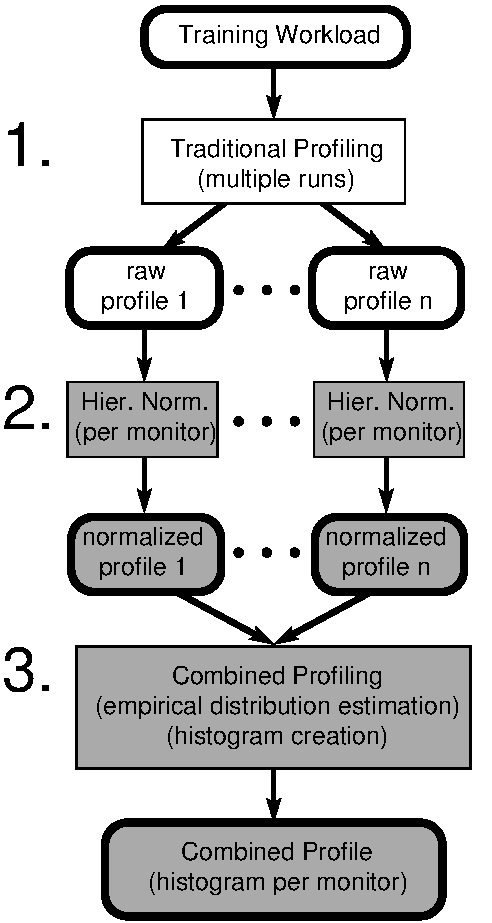
\includegraphics[width=2in]{Figures/cp-overview}
%  \caption{Three phases of combined profiling: 1) profile each input, 2) normalize each profile, and 3) combine the profiles into %a distribution model.}
%  \label{fig:cp-overview}
%\end{figure}

\CP\ and \HN\ have been presented in previous 
work~\cite{BerubeICPE11,BerubeISPASS12}. % However, this presentation
%clarifies and expands on previous versions, particularly the
%description of \CP's histograms in \refSection{cp:empirical} and the
%discussion of queries in \refSection{cp:queries}.
However, a clearer and expanded version, based on previous versions, can
be found in ~\cite{BerubePhD}, particularly the
description of \CP's histograms and the discussion of queries

%\refSection{cp:design} discusses the design of \CP, and the details of
%the technique are presented in \refSection{cp:empirical}.  \CP\ is
%widely applicable; \refSection{cp:extend} briefly discusses the use
%of \CP\ with additional forms of profiling.

%\begin{figure*}[h!]  % fullpage figures should always be at the top
%  \centering
%
%  \makebox[\linewidth][t]{
%  %  \centering  % centering does not seem to be working inside the box...
%
%    \subfigure[A control flow graph.  Edges are labeled with the raw
%      frequencies for \{P1, P2, P3\}.  The probabilities that the left
%      branch is taken from nodes $A$ and $B$ are listed in the
%      adjacent boxes.]{
%      \label{fig:motivate:cfg}
%      \begin{minipage}[b]{0.48\textwidth}
%        \centering
%        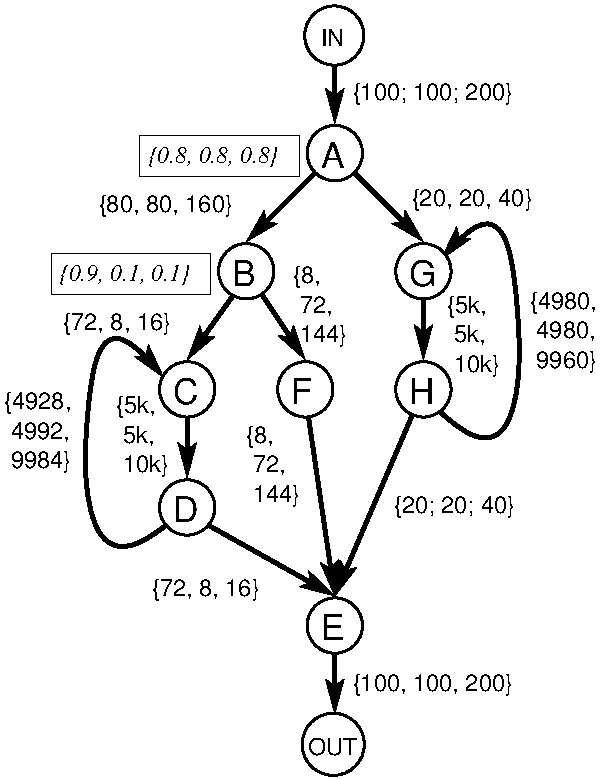
\includegraphics[width=\textwidth]{Figures/motivate}
%      \end{minipage}
%    } % end subfigure a 
%    \subfigure[The edge-dominator tree for \refFigure{fig:motivate:cfg}.]{
%      \label{fig:motivate:domtree}
%      \begin{minipage}[b]{0.48\textwidth}
%        \centering
%        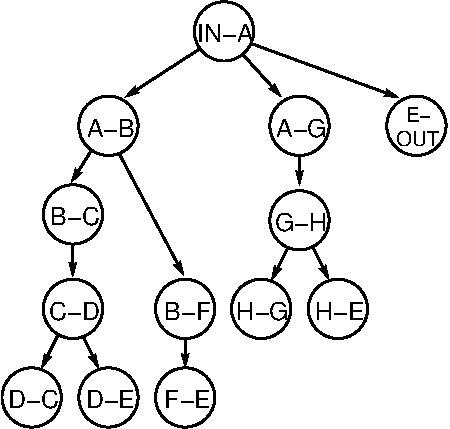
\includegraphics[width=\textwidth]{Figures/domtree}
%        \vspace{0.25in}
%      \end{minipage}
%    } % end subfigure b
%  }\\ % end makebox
%
%%    \hspace{0.15in} % Space between the figures; push table to right
%%                    % margin (compensates for lack of centering...)
%    
%    \subfigure[Profiles P1, P2 and P3 show raw edge frequency counts.
%      P1', P2', and P3' are hierarchically-normalized profiles suitable
%      for combined profiling.]{
%      \centering
%      \label{fig:motivate:eprof} 
%      \begin{minipage}[b]{\linewidth}
%        \centering
%%        \scriptsize
%        % The table will *JUST* fit in a column if it is enclosed by
%        % \begin{small}.  This would allow a 1-col stacked figure.
%        

% the \hspace is a trick to reduce the space taken by the empty column
% between section of the table (vs just leaving it empty)
\begin{tabular}{r@{$\rightarrow$}lr@{$\rightarrow$}lr@{\hspace{0.01in}}rrrr@{\hspace{0.01in}}rrr}

\multicolumn{2}{c}{} & \multicolumn{2}{c}{} 
  & & \multicolumn{3}{c}{\bf Raw}
  & & \multicolumn{3}{c}{\bf Normalized} \\  \cline{6-8} \cline{10-12}
\multicolumn{2}{c}{\bf Edge} \T & \multicolumn{2}{c}{\bf Dom}
  & & {\bf P1}  & {\bf P2}  & {\bf P3}
  & & {\bf P1'} & {\bf P2'} & {\bf P3'} \\ \hline

IN&A \T & \multicolumn{2}{c}{} 
             &&   100   & 100   & 200     &&   1.0  & 1.0 & 1.0 \\
A&B   & IN&A &&   80    & 80    & 160     &&   0.8  & 0.8 & 0.8 \\
A&G   & IN&A &&   20    & 20    & 40      &&   0.2  & 0.2 & 0.2 \\
G&H   & A&G  &&   5,000 & 5,000 & 10,000  &&   250  & 250 & 250 \\
H&G   & G&H  &&   4,980 & 4,980 & 9,960   &&   249  & 249 & 249 \\
H&E   & G&H  &&   20    & 20    & 40      &&   4.0e-3  & 4.0e-3 & 4.0e-3 \\
B&C   & A&B  &&   72    & 8     & 16      &&   0.9  & 0.1 & 0.1 \\
C&D   & B&C  &&   5,000 & 5,000 & 10,000  &&   69.4 & 625 & 625 \\
D&C   & C&D  &&   4,928 & 4,992 & 9,984   &&   1.0  & 1.0 & 1.0 \\
D&E   & C&D  &&   72    & 8     & 16      &&   1.4e-2  & 1.6e-3 & 1.6e-3 \\
B&F   & A&B  &&   8     & 72    & 144     &&   0.1  & 0.9 & 0.9 \\
F&E   & B&F  &&   8     & 72    & 144     &&   1.0  & 1.0 & 1.0 \\
E&OUT & IN&A &&   100   & 100   & 200     &&   1.0  & 1.0 & 1.0 \\ \hline

\end{tabular}
\\
%        ~ % without this space on a new line, the minipage has no
%          % actual line of text, and the alignment of the subfigures
%          % gets all screwed up.
%%        \vspace{0.25in}  % push the table up from the bottom of the figure
%      \end{minipage}
%    } % end subfigure c
%
%  \caption{The \CFG\ and  edge-dominator tree of a procedure, with three possible edge profiles}
%  \label{fig:motivate}
%\end{figure*}


\CP\ ~\cite{BerubePhD} provides a data representation for profile information, but does
not specify the semantics of the information stored in the combined
profile.  Raw profiles cannot be combined naively. %To illustrate this
%point, \refFigure{fig:motivate:cfg} presents a \CFG\, and the table in
%\refFigure{fig:motivate:eprof} provides the edge frequencies observed
%for three profiles: P1, P2, and P3. The numbers within the rectangles
%are the probabilities for edges A$\rightarrow$B and
%B$\rightarrow$C. First note that averaging values across profiles is
%misleading because it can easily characterize behavior in a way that
%does not correspond to any individual profile; The average branch
%probability at B is 0.37, hiding its strongly biased behavior.  In all
%three profiles, the probability of entering the G-H loop from A is
%0.2.  The loop trip counts for P1 and P2 are identical, but the
%probability of entering the C$\rightarrow$D loop from B is 0.9 in P1
%and 0.1 in P2.  P3 is identical to P2, except that all edge counts are
%doubled.  Therefore, P2 and P3 are essentially the same profile; if
%they were combined, the resulting profile should not show any
%variation in program behavior.  However, if the two raw frequencies
%for an edge such as G$\rightarrow$H were combined into a histogram,
%the values 5,000 and 10,000 would not suggest this consistent
%behavior.

%On the other hand, the raw frequencies for edge C$\rightarrow$D in
%P1 and P2 are both 5,000, but P1 enters the loop much more frequently
%than P2 due to the 0.9 vs 0.1 branch probability at B.  Therefore,
%the average trip count of the loop in P1 is much lower (69.4) than in
%P2 (625). In this case, histogramming the raw frequencies
%suggests consistent behavior for the loop, which is misleading.

\subsection{Hierarchical Normalization}
\label{cp:hn}

There is a problem when pairs of measurements are taken under different
conditions.  Thus, when
combining these measurements, all values recorded for a monitor must
be normalized relative to a common fixed reference.  {\em Hierarchical
  normalization} (\HN) ~\cite{BerubePhD} is a profile semantic designed for use with
\CP\ that achieves this goal by decomposing a \CFG\ into a hierarchy
of dominating regions.
%The results of using \HN\ for the profiles in
%\refFigure{fig:motivate:eprof} are shown in the right portion of the
%table.  As desired, P2 and P3 are identical, and the differences in
%loop trip count between P1 and P2 are identified.

%\HN\ is presented for vertex profiling.
\HN\ is presented for edge profiling.  Vertex profiles are treated
identically, but use the domination relationships between vertexes
instead of edges.  Domination is usually defined in terms of vertexes.
In order to use an existing implementation of a vertex dominator-tree
algorithm with edge profiles, use the line graph of the \CFG\ instead of
the \CFG\ itself.  The line graph contains one vertex for each edge in
the \CFG, and edges in the line graph correspond to adjacencies
between the edges of the \CFG.
%This technique may be similarly applied to a call-graph.

Decomposing a \CFG\ into a hierarchy of dominating regions to enable
\HN\ is achieved by constructing its dominator tree. Each edge in the
\CFG\ is represented by a node in the dominator tree.  Denote the
immediate proper dominator of \CFG\ edge $e$ by $dom(e)$.  Each non-leaf
node $n(e)$ in the dominator tree is the head of a region $G_e$, which,
by construction, encompasses any regions entered through descendants of
$e$.  To prepare a raw profile for combination with other profiles,
the frequency $f_e$ of each non-root node $n(e)$ is normalized against
the frequency of its immediate proper dominator, $f_{dom(e)}$.
The ratio of these two frequencies is invariant when a branch
probability or loop iteration count is (dynamically) constant.
This process also prevents variable behavior in an outer loop from masking
consistent behaviors within the loop.  Normalization proceeds in a
bottom-up traversal of the dominator tree, so that the head of a
region is normalized to its immediate dominator only after all of its
descendents have been normalized.  The root of the dominator tree,
\ie, the edge representing entry into the procedure, is assigned a
``normalized'' value of 1.

%In order to understand the capabilities and limitations of a
%statistical model incorporating \HN, and to use it correctly, the
%model must be precisely defined.  Therefore, let $\fancy{F}_e$ and
%$\fancy{F}_{dom(e)}$ be random variables for the raw frequencies of
%$e$ and $dom(e)$, respectively.  Define a new random variable $Y_e =
%\frac{\fancy{F}_e}{\fancy{F}_{dom(e)}}$, which is the frequency of
%edge $e$ with respect to its dominator.  The raw profile from run 1 of
%the program records $f_{dom(e)}^1$ and $f_e^1$, the observed
%frequencies of the two nodes over that run.  One sample of $Y_e$,
%$y_e^1 = \frac{f_e^1}{f_{dom(e)}^1}$ is calculated as the
%hierarchically normalized value for $e$.  Over $k$ runs, $k$ samples
%$y_e^1, y_e^2, ..., y_e^k$ are added to the histogram of $R_e$.  Thus,
%the histogram of monitor $R_e$ is an approximation for the true
%probability density $R_e^*$ ~\cite{BerubePhD}:

%$$ \P(R_e \le \theta) \approx \P(R_e^* \le \theta) = \P \left(Y \le \theta\right) = \P \left(\frac{\fancy{F}_e}{\fancy{F}_{dom(e)}} \le \theta \right)$$

%$$ \P(\alpha \le R_e \le \beta) \approx \P(\alpha \le R_e^* \le \beta) = \P \left(\alpha \le Y \le \beta\right) = \P \left( \alpha \le \frac{\fancy{F}_e}{\fancy{F}_{dom(e)}} \le \beta \right)$$

%$ \int_0^{\theta} R_e \approx \int_0^{\theta} R_e^* = \P \left(Y \le \theta\right) = \P \left(\frac{\fancy{F}_e}{\fancy{F}_{dom(e)}} \le \theta \right)$$




\subsection{Denormalization}
\label{cp:denorm}

The properties of a monitor $R_a$ can only be directly compared to
those of a monitor $R_b$ when $dom(a) = dom(b)$.  However, more
generalized reasoning about $R_a$ may be needed when considering code
transformations.  Similarly, when code is moved by a transformation,
its profile information must be correctly updated. {\it
  Denormalization} reverses the effects of hierarchical normalization
to lift monitors out of nested domination regions by marginalizing-out
the distribution of the dominators above which they are lifted.
Denormalization is a heuristic method rather than an exact statistical
inference because it assumes statistical independence between monitors.
%inference because it assumes statistical\footnote{$R_i$,$R_j$ are
%  independent iff $ \forall i,j:\P(R_i=i,R_j=j) = \P(R_i=i)\P(R_j=j)$.
%  Control-flow equivalence implies independence. Independence does not
%  hold in most other cases.}  independence between monitors.

%Consider first the hierarchically-normalized raw profiles in
%\refFigure{fig:motivate}.  Intuitively, the expected execution count
%of node $F$ for a single execution through the graph is calculated:
%\begin{eqnarray*}
%\mathrm{BP}_l(A) &=& \left(\frac{f_{A\leftarrow B}}{f_{A\leftarrow B} + f_{A\leftarrow G}}\right) \\
%\mathrm{BP}_r(B) &=& \left(\frac{f_{B\leftarrow F}}{f_{B\leftarrow C} + f_{B\leftarrow F}}\right) \\
%\E[f_F] &=& \E[R_{IN\leftarrow A} \times \mathrm{BP}_l(A) \times \mathrm{BP}_r(B)]\\
%\mathrm{P1}:\E[f_F] &=& 1.0 \times 0.80 \times 0.90 = 0.72 \\
%\mathrm{P2, P3}:\E[f_F] &=& 1.0 \times 0.80 \times 0.10 = 0.08
%\end{eqnarray*}
%where $\mathrm{BP}_d(n)$ is the probability of a branch going in
%direction $d$ (either (l)eft or (r)ight) from node $n$.  However, even
%a single raw profile is a statistical model. Thus, the calculation
%above assumes that the edge frequencies are independent.
  
%With the same assumption, the same approach can be used with a \CP.
%Thus, for the \CP\ built from P1, P2 and P3:
%$$ \E[f_F] = 1.0 \times 0.8 \times \left(\frac{0.9+0.1+0.1}{3}\right) = 0.29 $$ 
%which is the average of the expected frequencies.

%The mean is a special case of marginalization; independence allows the
%joint distribution to be broken into the product of individual
%distributions, where the expectation associates over the product,
%simplifying the calculation to the product of means seen above.  Thus,
%to recover an ``absolute'' expected execution count from an
%\HN\ \CProf, multiply the means of each monitor up the dominator tree
%to the procedure entry.  Then, multiply by the expected invocation
%frequency of the procedure (possibly using this technique over a
%\CG\ \CProf).  Denormalization is this process of multiplying monitors
%along a path in the dominator tree.  The mean is a special case of
%denormalization because it does not require the distribution of
%monitor values.  The general denormalization technique is formally
%presented in the remainder of this section.

%Let $R_a$ and $R_b$ be monitors from the same \CFG.  Let
%$\mathit{dom}^i(R_a)$ be the $i^{th}$ most-immediate proper dominator
%of $R_a$.  The least-common dominator of $R_a$ and $R_b$ is $R_d =
%\mathit{dom}^j(R_a) = \mathit{dom}^k(R_b)$, where there is no monitor
%$R_n$ such that $R_d$ properly dominates $R_n$, and $R_n$ dominates
%both $R_a$ and $R_b$.  Denormalizing $R_a$ from the region dominated
%by $\mathit{dom}(R_a)$ to the region dominated by $R_d$ is achieved by
%walking up the dominator tree.  Let $\widehat{R_n^{-i}}$ be the
%denormalized distribution when $R_n$ is lifted above $dom^i(n)$.
%$\widehat{R_n^{-1}}$ is created by multiplying together the histograms
%$H_n$ and $H_{dom(n)}$. Denormalization can be applied to $R_a$ and
%$R_b$ recursively to produce the desired $\widehat{R_a^{-j}}$ and
%$\widehat{R_b^{-k}}$, which can be compared ~\cite{BerubePhD}.

%The computation of $\widehat{R_n^{-i}}$ takes $O(ib^2)$ time, assuming
%that all histograms use $b$ bins.  The number of bins is chosen by the
%user. There is a tradeoff between accuracy and precision on one hand
%and memory space and computation time on the other.

%\begin{figure}
%  \centering
%  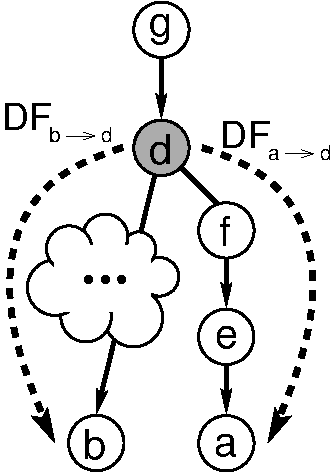
\includegraphics[width=0.3\linewidth]{Figures/denormalize}
%  \caption{Denormalization of $R_a$ and $R_b$ with respect to their
%    least-common dominator $R_d$.  Dashed lines show the path over
%    which the marginalized histograms are computed.}
%  \label{fig:denormalize}
%\end{figure}

%\refFigure{fig:denormalize} shows a dominator tree containing the
%nodes $a$ and $b$ and their least common dominator $d$, which is
%shaded.  The dashed lines illustrate the paths followed, in the
%dominator tree, to compute the denormalization. Nodes $f$ and $e$ are
%in the path from $d$ to $a$ and there might be other nodes in the path
%from $d$ to $b$.  Thus, $R_d = \mathit{dom}^3(R_a)$, and the histogram
%for $\widehat{R_a^{-3}}$ is calculated:
%$$ \widehat{H_a^{-3}} = H_a \times H_e \times H_f \times H_d $$


\subsection{Queries}
\label{cp:queries}

In an AOT compiler, profiles are used to predict program behavior.
Thus, raw profiles are statistical models that use a single sample to
answer exactly one question: {\em ``What is the expected frequency of
  X?''}  where X is an edge or path in a \CFG\ or a Call Graph (\CG).
A \CP\ is a much richer statistical model that can answer a wide range
of queries about the measured program behavior.  The implementation of
\CP\ used in this work provides the following statistical queries as
methods of a monitor's histogram:
\begin{description}

\item[$H.\mathrm{min}, H.\mathrm{max}$]: \\
%  The maximum and non-zero
%  minimum monitor value observed, as in ~\cite{BerubePhD}.

\item[$H.\mathrm{mean}(\mathit{incl0s})$]: \\
%  The true weighted average of
%  observed monitor values.  If {\it incl0s} is true, count raw
%  profiles where the monitor did not execute as 0-valued observations,
%  as in ~\cite{BerubePhD}.

\item[$H.\mathrm{stdev}(\mathit{incl0s})$]: \\
%  The true weighted standard
%  deviation of observed monitor values.  If {\it incl0s} is true,
%  count raw profiles where the monitor did not execute as 0-valued
%  observations, as in ~\cite{BerubePhD}.

\item[$H.\mathrm{estProbLessThan}(v)$]: \\
%  Estimates the value of the
%  monitor's CDF at $v$, \ie, $\P(R \le v)$.  The estimation is based
%  on the assumed uniform distribution of bins.

\item[$H.\mathrm{quantile(q)}$]: \\
%  For $0 \le q \le 1$, estimates the
%  (minimum) value $v$ at the point where the monitor's CDF equals $q$,
%  \ie, $v$ when $\P(R \le v) = q$.  The estimation is based on the
%  assumed uniform distribution of bins.

\item[$H.\mathrm{applyOnRange}(F(w,v),\mathit{vmin},\mathit{vmax})$]: \\
%  Computes the sum of applying the function $F(w,v)$ to the impulses
%  of the histogram in the range $[\mathit{vmin}, \mathit{vmax}]$, as
%  with the multiplication of histograms in ~\cite{BerubePhD}.
%  For bins that partially overlap the range, the impulse's weight is
%  proportional to the overlap of the bin with the range, and the
%  impulse's value is the midpoint of the overlapping range.

\item[$H.\mathrm{applyOnQuantile}(F(w,v),\mathit{qmin},\mathit{qmax})$]: \\
%  Like applyOnRange, but the range is set using the values associated
%  with the quantile points {\it qmin} and {\it qmax}.

\item[$H.\mathrm{coverage}$]: \\
%  The probability of the monitor executing
%  in a run of the program, computed as $\frac{H.W}{H.\mathit{TW}}$.

\item[$H.\mathrm{span}$]: \\
%  The ratio between the range of the histogram
%  and its maximum value, computed as $\frac{H.\mathrm{max} -
%    H.\mathrm{min}}{H.\mathrm{max}}$.

\end{description}


The mean value of a monitor is analogous to the value provided by a
single raw profile, and provides the desired substitutability of a
\CProf\ for a raw profile in existing \FDO\ transformations.

\REM{ along with the standard deviation and minimum and maximum
  values.  Furthermore, \CP\ can estimate from a monitor's Cumulative
  Distribution Function (CDF) the probability that the monitor is
  within a (possibly half-bounded) range.  Conversely, the inverse CDF
  provides estimates of the thresholds corresponding to a given
  quantity of probability mass.  For example, the inverse CDF
  facilitates estimating the median value of a monitor.
}

%The additional statistical information provided by a \CProf\ allows an
%\FDO\ heuristic to quantify the expected trade-offs between various
%workload-performance measurements, such as between the impact on the
%5\%-quantile (nearly worst-case) or the average impact on the
%5\%--95\%-quantile range (omitting potential outliers).  In some
%transformations, the order in which candidates are considered is
%important~\cite{ChakrabartiCGO06}.  \CP\ allows a sorting function to
%use, for example, both the mean and the standard deviation of the
%candidates in order to prioritize low-variance opportunities.
%Behavior variation should not, by itself, inhibit
%optimization. Rather, 
\CP\ enables the accurate assessment of the
potential performance impact of transformations informed by
variable-behavior monitors in a variety of ways, and with adjustable
confidence in the result. Concrete examples of this kind of analysis
are provided by the implementation of an \FDO\ inliner using
\CP\ described in \cite{BerubePhD}.


\subsection{Extensions and Alternative Usage}
\label{cp:extend}

The empirical-distribution methodology of \CP\ is orthogonal to the
techniques used to collect raw profiles.  \CP\ is applicable whenever
multiple profile instances are collected, including intra-run
phase-based profiles, profiles collected from hardware
performance-counter, and sampled profiles.  The main issue when
combining profiles is how normalization should be done in order to
preserve program-behavior characteristics.

\subsubsection{\CFG\ Paths}

%\begin{figure}
%  \centering
%  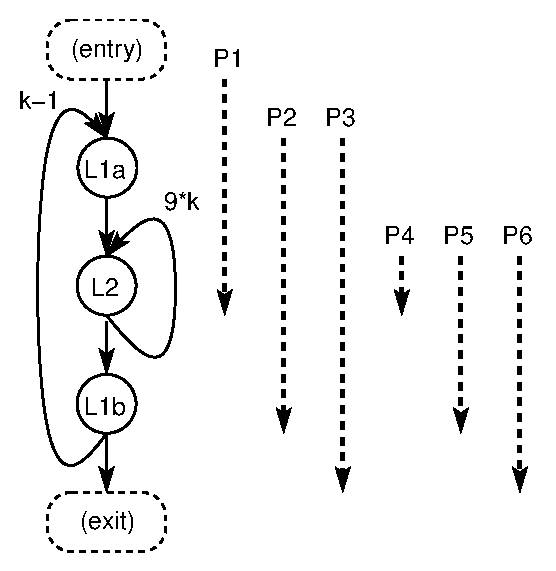
\includegraphics[width=0.50\linewidth]{Figures/pathnorm}
%  \caption{Some sub-paths through a nested loop. The outer loop
%    $L_1$ iterates a total of $k$ times; the inner loop $L_2$ iterates 10
%    times per iteration of $L_1$.}
%  \label{fig:pathnorm}
%\end{figure}

An algorithm that collects path profiling in a program that contains
loops must break cycles.  The most commonly used technique to break
such cycles is due to Ball and Larus~\cite{BallLarusMICRO96}. Given a
simple loop, the main idea is to replace the back edge with a set of
sub-paths that include (a) a path from a point outside the loop to the
end of the first iteration, (b) a path from the loop entry point to a
point outside the loop, and (c) a path from the entry point to the
exit point in the loop.
% \refFigure{fig:pathnorm} illustrates some of
%the paths inserted to replace the two back edges in a double-nested
%loop.

Hierarchical normalization must be adapted to work with paths because
there are no dominance relationships between paths. Consider two runs
of a double-nested loop, where the outer
loop $L_1$ iterates a total of $k=10,000$ times in the first run, and
$k=100$ times in the second run.  In both cases the inner loop $L_2$
iterates 10 times per iteration of $L_1$.  A combined profile should
identify the path of execution within $L_1$ as consistent across runs,
but should indicate that the frequency of the paths into and out of
$L_1$ vary significantly from run to run. The solution is to normalize
path frequencies with respect to the frequency of the vertex that
starts the path.  For instance, P4 should be normalized to the
frequency of $L_2$ to factor out $k$ and preserve the constant nature
of the inner loop.


%\subsubsection{Program Call-Graphs}

%Combined profiling can easily be extended to call-graphs
%(\CG)\footnote{We do not attempt to extend \CP\ to inter-procedural
%  paths~\cite{MelskiPhd02}.}.  Profiling a \CG\ gathers information
%about the frequency of inter-procedural calls.  A \CG\ can be
%represented in multiple ways.  For instance, a single edge may
%represent all calls from a procedure \funcname{foo()} to a procedure
%\funcname{bar()}.  Alternatively, there may be a separate edge for
%each call-site in \funcname{foo()} that targets \funcname{bar()}. If
%context-sensitivity is included, there are several alternatives to
%keep track of the execution path that leads to a call from
%\funcname{foo()} to \funcname{bar()}.  A common solution is to keep
%track of the $k$ most recent calls on the stack when the call from
%\funcname{foo()} to \funcname{bar()} occurs~\cite{MightPLDI10}.  This
%sequence of calls is called a {\em call string}.

% \pb{Changed based on our discussion for inlining}
%Unlike a \CFG, a \CG\ is not a well-structured graph.  Consequently,
%the dominator tree is often very wide and shallow, which limits the
%utility of applying \HN\ to the full \CG.  Instead, we propose that
%\CG\ monitors are normalized with respect to the invocation frequency
%of the procedure where the behavior originates. In the case of
%\CG\ profiles that do not use context sensitivity, call frequencies
%are normalized against the caller's frequency.  Likewise, when
%context-sensitivity is used to collect a \CG\ profile, call-string
%frequencies are normalized against the frequency of the caller of the
%first call in the string.  The combined profile then provides a
%conditional distribution describing the expected frequency of
%following a call or call string, given that the start of the call
%string has been reached.


%\subsubsection{Value Profiling}

%A monitor $R$ for value profiling observes the run-time values of a
%variable at a specific program point in order to enable specialization
%transformations~\cite{Calder97}.  Each profiling run produces a
%histogram of the frequency of observed values of the variable.
%However, since a variable could potentially take very many different
%values over a program run, a caching technique is used to estimate the
%frequency of the $n$ most frequent values.  Since a value profile is
%completely local to a single program point, there is no hierarchy over
%which to normalize; normalization simply requires converting the
%frequency for each value $v$, $f(v)$, into a proportion of
%the total number of observations, $\P(v)$ (\ie, the probability of
%observing $v$).  The \CProf\ for value profiling then creates a
%histogram for each frequently-observed $v$ over the $\P(v)$ of each
%run.  Thus, the \CProf\ identifies the frequent values of $R$, and the
%distribution of the likelihood of observing each value.  If the set of
%frequent values is not consistent across runs, less-likely values may
%need to be pruned from the \CProf, or the variable may simply be
%marked as unsuitable for specialization.

%\subsubsection{Profiling Granularity}

%This work assumes that \CP\ will combine input profiles from complete,
%single, program runs.  However, the input profiles can have arbitrary
%granularity.  For instance, \CP\ could combine \CFG\ profiles from
%each separate invocation of a function (a finer temporal granularity).
%Similarly, each thread in a concurrent application could contribute a
%separate raw profile for combination into a multi-threaded \CProf\ for
%a single run (thread-level granularity).  In conjunction with phase
%detection, a \CProf\ could be build to represent behavior variation
%between fine-grained program phases.  Conversely, long-running server
%applications could periodically commit profile information to
%a \CProf\ to model program behavior variation over different times of
%day or even different days of the week.


%\REM{
%\section{old stuff}
%Other stuff that is obvious or interesting or has come up in the
%course of research and has been put aside as beyond the scope of this
%work:
%\begin{itemize}
%\item Keep profiles across code changes?
%\item Finer-grained profiling (candidacy: scope)
%\item Value profiling: histograms-of-histograms
%\item \todo{CG profiling, all variations: expand on ISPASS'11}
%\item Inter-procedural path profiling
%\end{itemize}
%}
